% Options for packages loaded elsewhere
\PassOptionsToPackage{unicode}{hyperref}
\PassOptionsToPackage{hyphens}{url}
\PassOptionsToPackage{dvipsnames,svgnames,x11names}{xcolor}
%
\documentclass[
  letterpaper,
  DIV=11,
  numbers=noendperiod]{scrartcl}

\usepackage{amsmath,amssymb}
\usepackage{iftex}
\ifPDFTeX
  \usepackage[T1]{fontenc}
  \usepackage[utf8]{inputenc}
  \usepackage{textcomp} % provide euro and other symbols
\else % if luatex or xetex
  \usepackage{unicode-math}
  \defaultfontfeatures{Scale=MatchLowercase}
  \defaultfontfeatures[\rmfamily]{Ligatures=TeX,Scale=1}
\fi
\usepackage{lmodern}
\ifPDFTeX\else  
    % xetex/luatex font selection
\fi
% Use upquote if available, for straight quotes in verbatim environments
\IfFileExists{upquote.sty}{\usepackage{upquote}}{}
\IfFileExists{microtype.sty}{% use microtype if available
  \usepackage[]{microtype}
  \UseMicrotypeSet[protrusion]{basicmath} % disable protrusion for tt fonts
}{}
\makeatletter
\@ifundefined{KOMAClassName}{% if non-KOMA class
  \IfFileExists{parskip.sty}{%
    \usepackage{parskip}
  }{% else
    \setlength{\parindent}{0pt}
    \setlength{\parskip}{6pt plus 2pt minus 1pt}}
}{% if KOMA class
  \KOMAoptions{parskip=half}}
\makeatother
\usepackage{xcolor}
\setlength{\emergencystretch}{3em} % prevent overfull lines
\setcounter{secnumdepth}{-\maxdimen} % remove section numbering
% Make \paragraph and \subparagraph free-standing
\ifx\paragraph\undefined\else
  \let\oldparagraph\paragraph
  \renewcommand{\paragraph}[1]{\oldparagraph{#1}\mbox{}}
\fi
\ifx\subparagraph\undefined\else
  \let\oldsubparagraph\subparagraph
  \renewcommand{\subparagraph}[1]{\oldsubparagraph{#1}\mbox{}}
\fi


\providecommand{\tightlist}{%
  \setlength{\itemsep}{0pt}\setlength{\parskip}{0pt}}\usepackage{longtable,booktabs,array}
\usepackage{calc} % for calculating minipage widths
% Correct order of tables after \paragraph or \subparagraph
\usepackage{etoolbox}
\makeatletter
\patchcmd\longtable{\par}{\if@noskipsec\mbox{}\fi\par}{}{}
\makeatother
% Allow footnotes in longtable head/foot
\IfFileExists{footnotehyper.sty}{\usepackage{footnotehyper}}{\usepackage{footnote}}
\makesavenoteenv{longtable}
\usepackage{graphicx}
\makeatletter
\def\maxwidth{\ifdim\Gin@nat@width>\linewidth\linewidth\else\Gin@nat@width\fi}
\def\maxheight{\ifdim\Gin@nat@height>\textheight\textheight\else\Gin@nat@height\fi}
\makeatother
% Scale images if necessary, so that they will not overflow the page
% margins by default, and it is still possible to overwrite the defaults
% using explicit options in \includegraphics[width, height, ...]{}
\setkeys{Gin}{width=\maxwidth,height=\maxheight,keepaspectratio}
% Set default figure placement to htbp
\makeatletter
\def\fps@figure{htbp}
\makeatother

\KOMAoption{captions}{tableheading}
\definecolor{hitsblue}{RGB}{0, 31, 73}
\makeatletter
\makeatother
\makeatletter
\makeatother
\makeatletter
\@ifpackageloaded{caption}{}{\usepackage{caption}}
\AtBeginDocument{%
\ifdefined\contentsname
  \renewcommand*\contentsname{Table of contents}
\else
  \newcommand\contentsname{Table of contents}
\fi
\ifdefined\listfigurename
  \renewcommand*\listfigurename{List of Figures}
\else
  \newcommand\listfigurename{List of Figures}
\fi
\ifdefined\listtablename
  \renewcommand*\listtablename{List of Tables}
\else
  \newcommand\listtablename{List of Tables}
\fi
\ifdefined\figurename
  \renewcommand*\figurename{Figure}
\else
  \newcommand\figurename{Figure}
\fi
\ifdefined\tablename
  \renewcommand*\tablename{Table}
\else
  \newcommand\tablename{Table}
\fi
}
\@ifpackageloaded{float}{}{\usepackage{float}}
\floatstyle{ruled}
\@ifundefined{c@chapter}{\newfloat{codelisting}{h}{lop}}{\newfloat{codelisting}{h}{lop}[chapter]}
\floatname{codelisting}{Listing}
\newcommand*\listoflistings{\listof{codelisting}{List of Listings}}
\makeatother
\makeatletter
\@ifpackageloaded{caption}{}{\usepackage{caption}}
\@ifpackageloaded{subcaption}{}{\usepackage{subcaption}}
\makeatother
\makeatletter
\@ifpackageloaded{tcolorbox}{}{\usepackage[skins,breakable]{tcolorbox}}
\makeatother
\makeatletter
\@ifundefined{shadecolor}{\definecolor{shadecolor}{rgb}{.97, .97, .97}}
\makeatother
\makeatletter
\makeatother
\makeatletter
\makeatother
\ifLuaTeX
  \usepackage{selnolig}  % disable illegal ligatures
\fi
\IfFileExists{bookmark.sty}{\usepackage{bookmark}}{\usepackage{hyperref}}
\IfFileExists{xurl.sty}{\usepackage{xurl}}{} % add URL line breaks if available
\urlstyle{same} % disable monospaced font for URLs
\hypersetup{
  pdftitle={MD and Reactions},
  pdfauthor={Eric Hartmann},
  pdfkeywords={template, demo},
  colorlinks=true,
  linkcolor={hitsblue},
  filecolor={Maroon},
  citecolor={Blue},
  urlcolor={hitsblue},
  pdfcreator={LaTeX via pandoc}}

\title{MD and Reactions}
\author{Eric Hartmann}
\date{2023-10-04}

\begin{document}
\maketitle
\ifdefined\Shaded\renewenvironment{Shaded}{\begin{tcolorbox}[frame hidden, boxrule=0pt, enhanced, sharp corners, interior hidden, breakable, borderline west={3pt}{0pt}{shadecolor}]}{\end{tcolorbox}}\fi

\hypertarget{kimmdy-structure-and-theory}{%
\subsection{KIMMDY structure and
theory}\label{kimmdy-structure-and-theory}}

\hypertarget{section}{%
\subsection{}\label{section}}

\hypertarget{section-1}{%
\subsection{}\label{section-1}}

\hypertarget{practice}{%
\section{Practice}\label{practice}}

\hypertarget{kimmdy-can-break-a-triplehelix-and-continue-simulating-for-a-bit}{%
\subsection{\texorpdfstring{KIMMDY can break a triplehelix (and continue
simulating for a
bit)}{KIMMDY can break a triplehelix   (and continue simulating for a bit)}}\label{kimmdy-can-break-a-triplehelix-and-continue-simulating-for-a-bit}}

\hypertarget{system-energy-is-continuous}{%
\subsection{System energy is
continuous}\label{system-energy-is-continuous}}

\texttt{kimmdy-analysis\ energy\ \textless{}run\_dir\textgreater{}\ -t\ Potential}

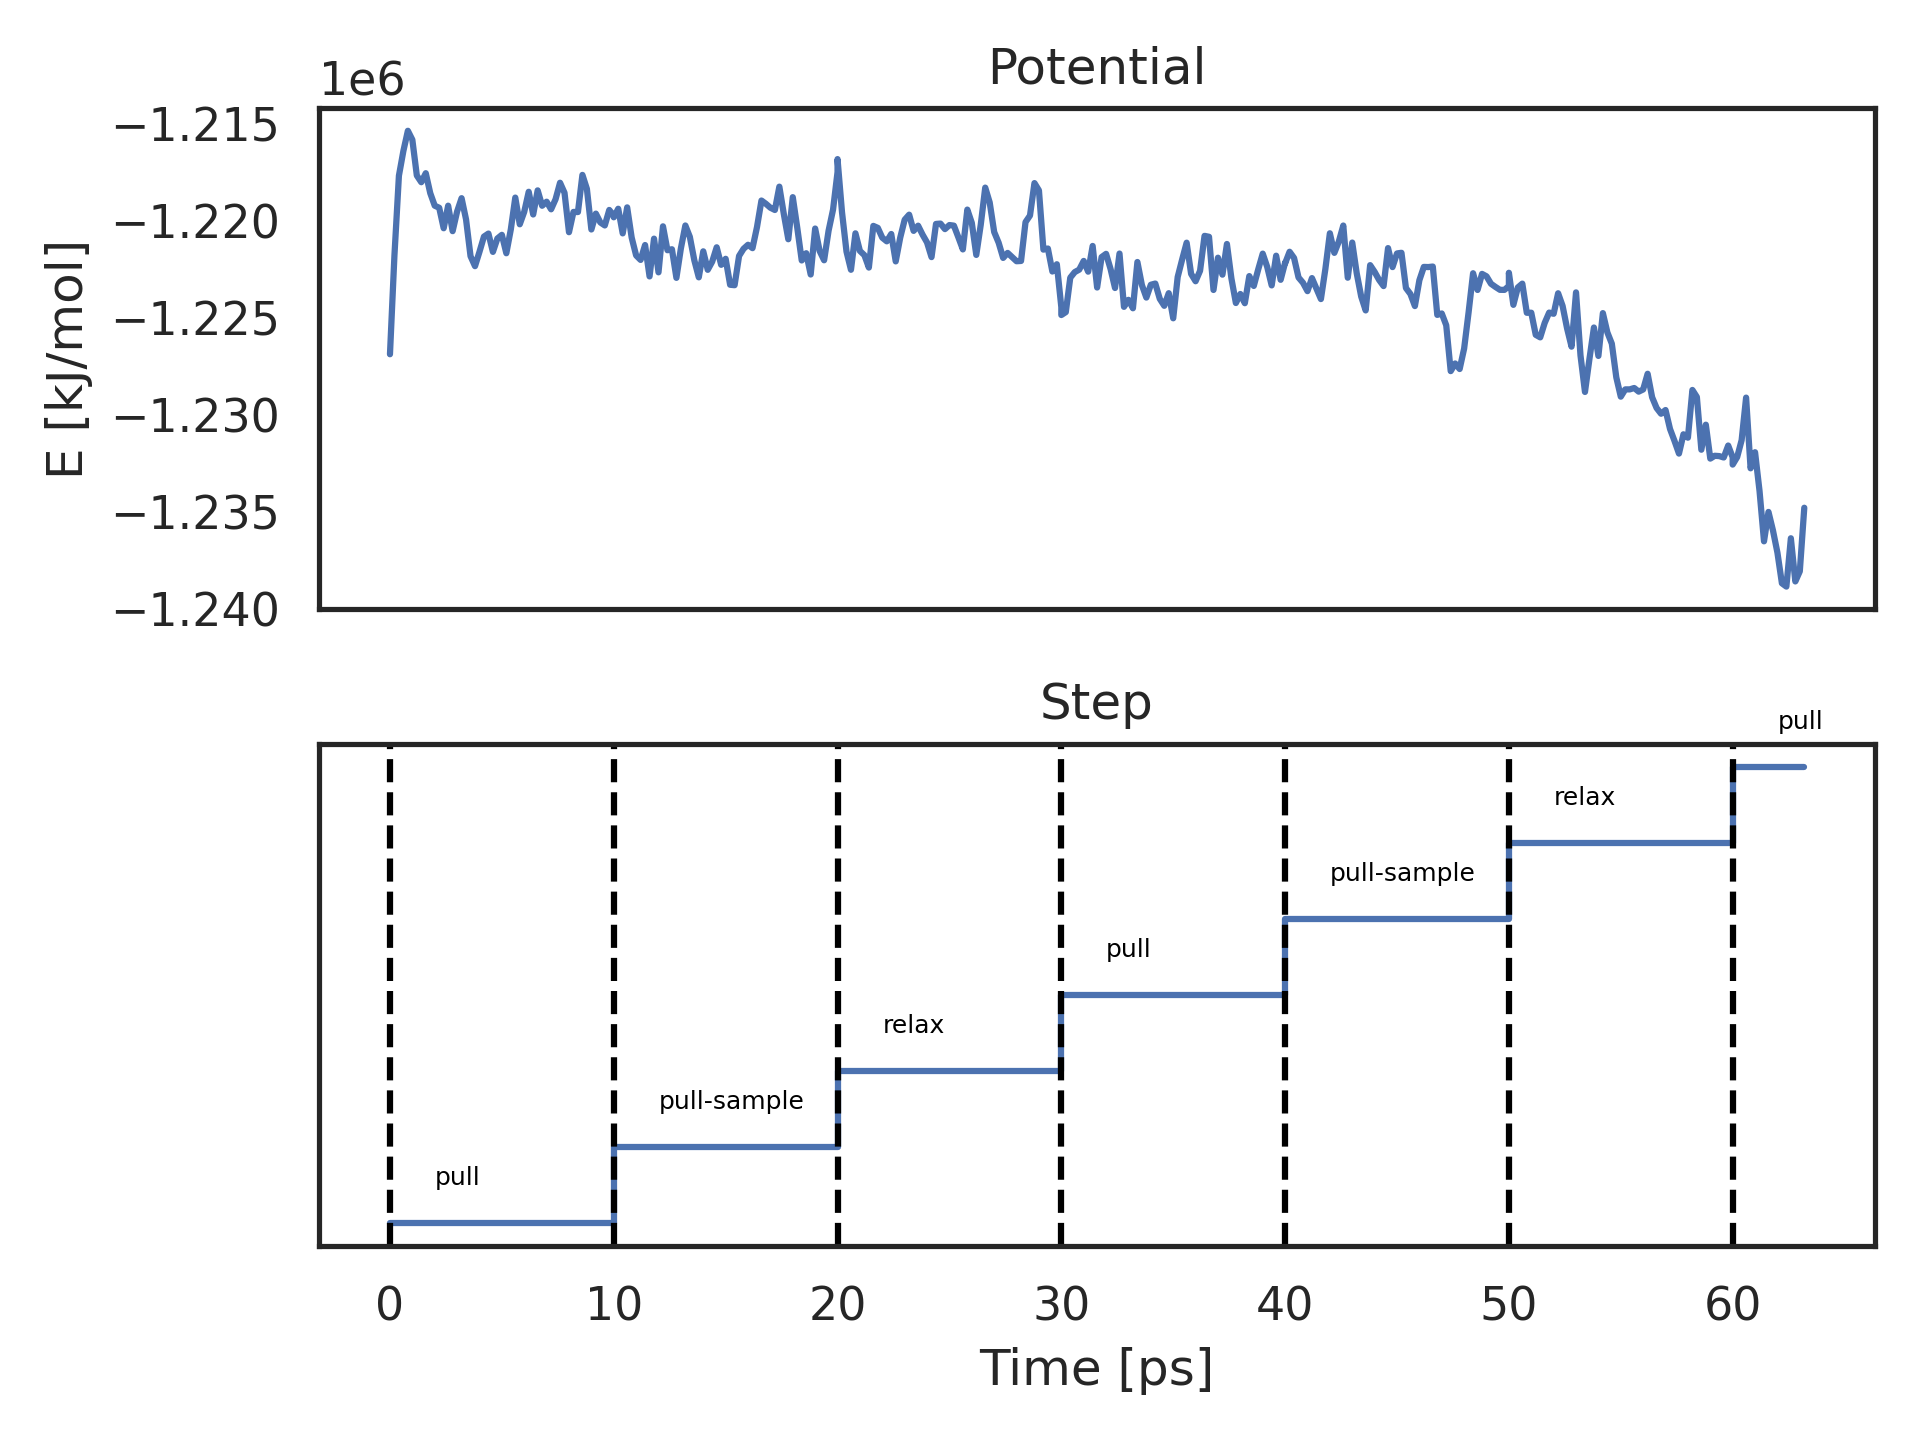
\includegraphics{www/tripelhelix_potential.png}

\hypertarget{intramolecular-energy-is-continuous}{%
\subsection{Intramolecular energy is
continuous}\label{intramolecular-energy-is-continuous}}

\texttt{kimmdy-analysis\ energy\ \textless{}run\_dir\textgreater{}\ -t\ 1\ Angle\ Proper-Dih.}

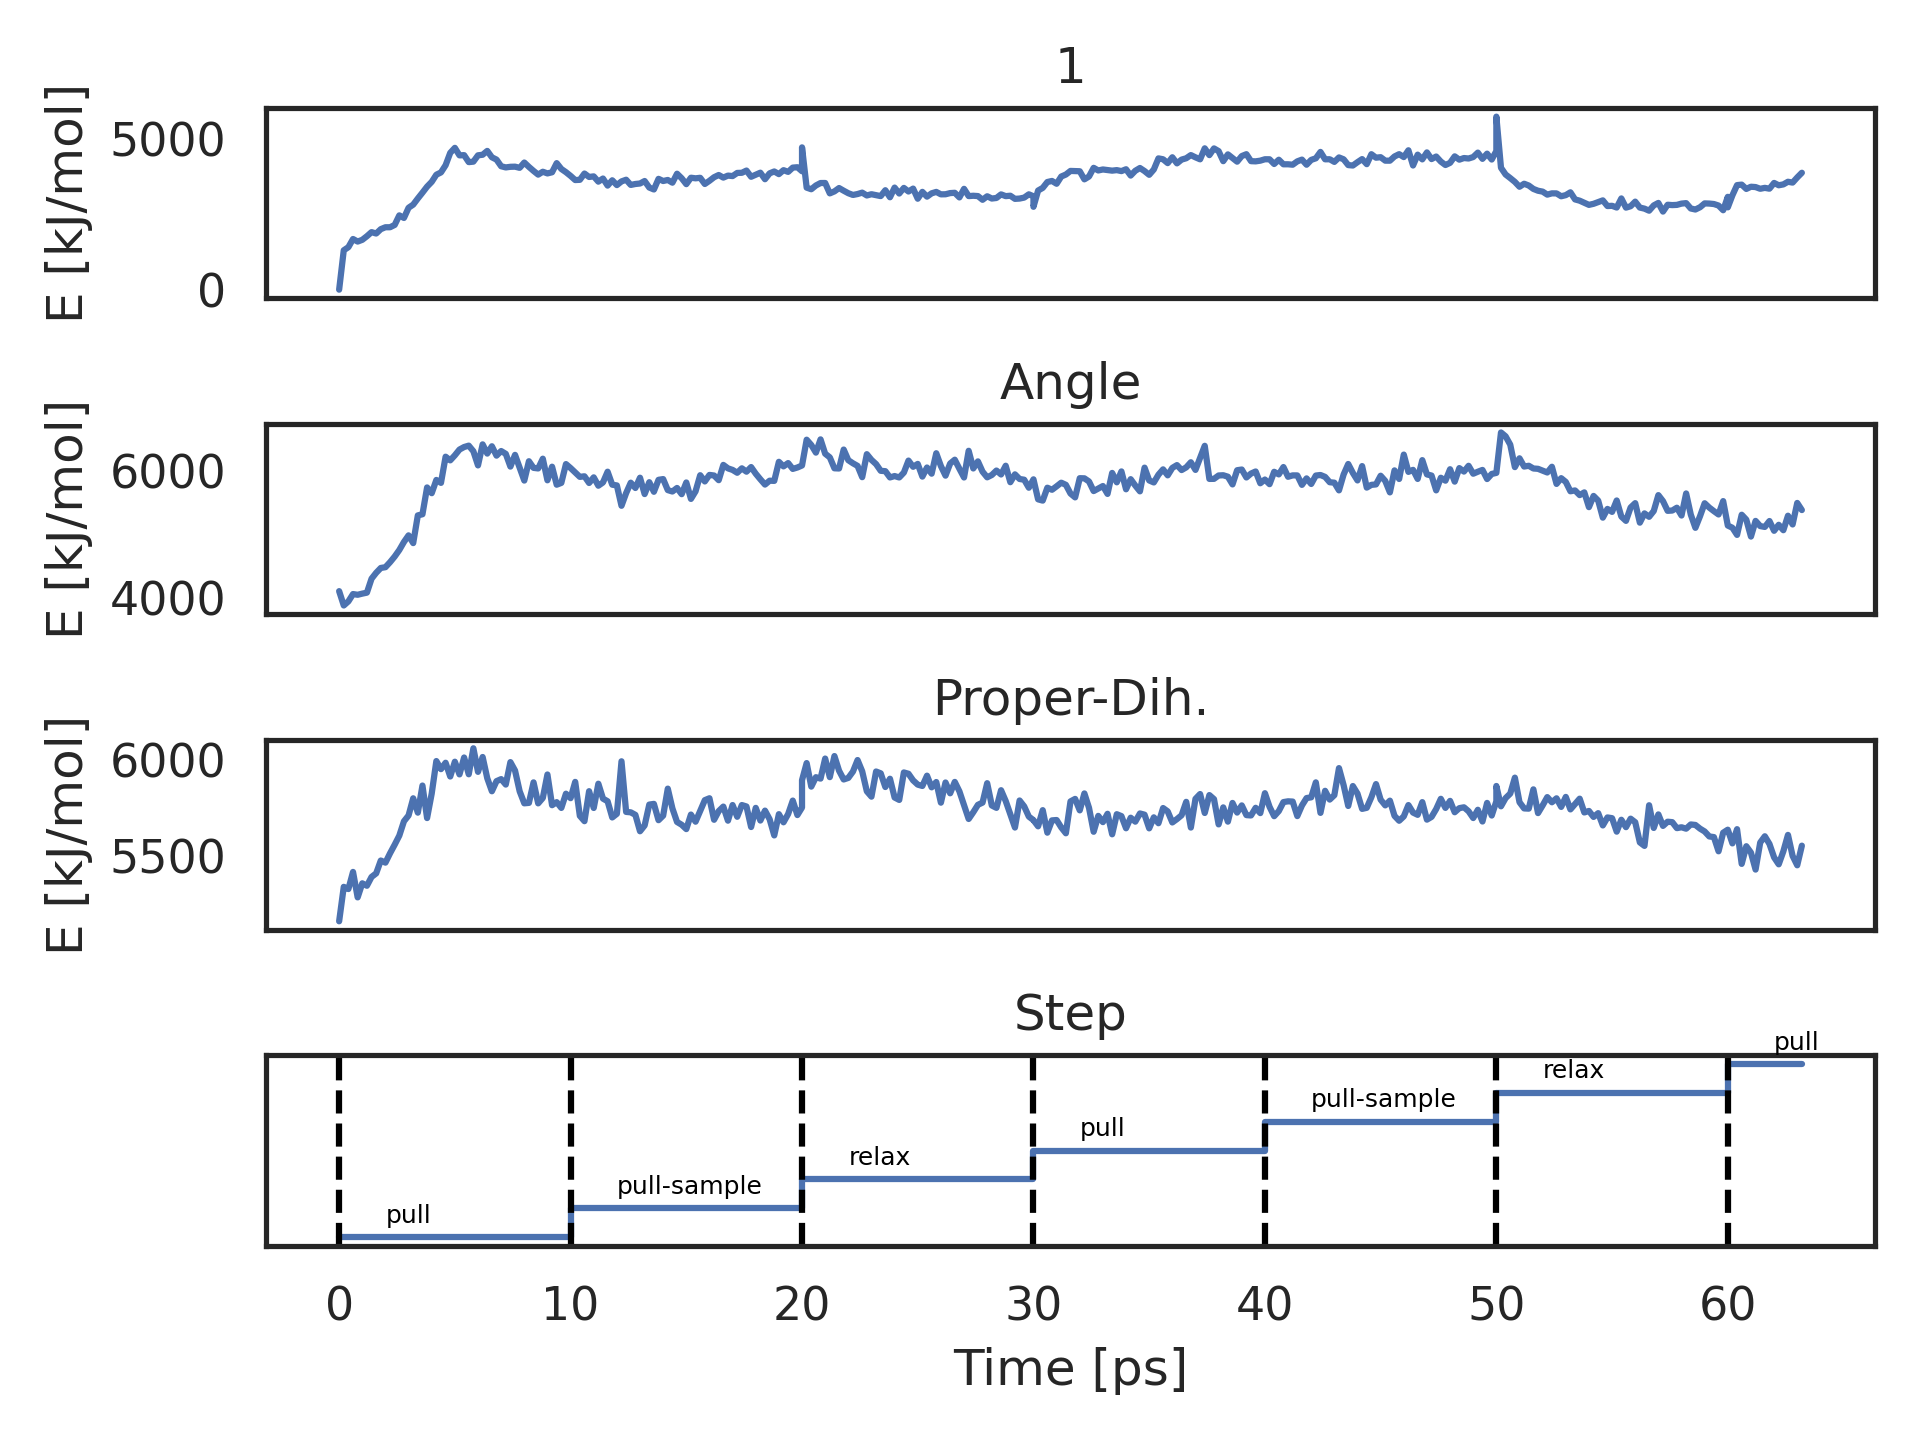
\includegraphics{www/tripelhelix_bonded.png}

\hypertarget{most-of-the-time-is-spend-on-md}{%
\subsection{Most of the time is spend on
MD}\label{most-of-the-time-is-spend-on-md}}

\texttt{kimmdy-analysis\ runtime\ \textless{}run\_dir\textgreater{}}

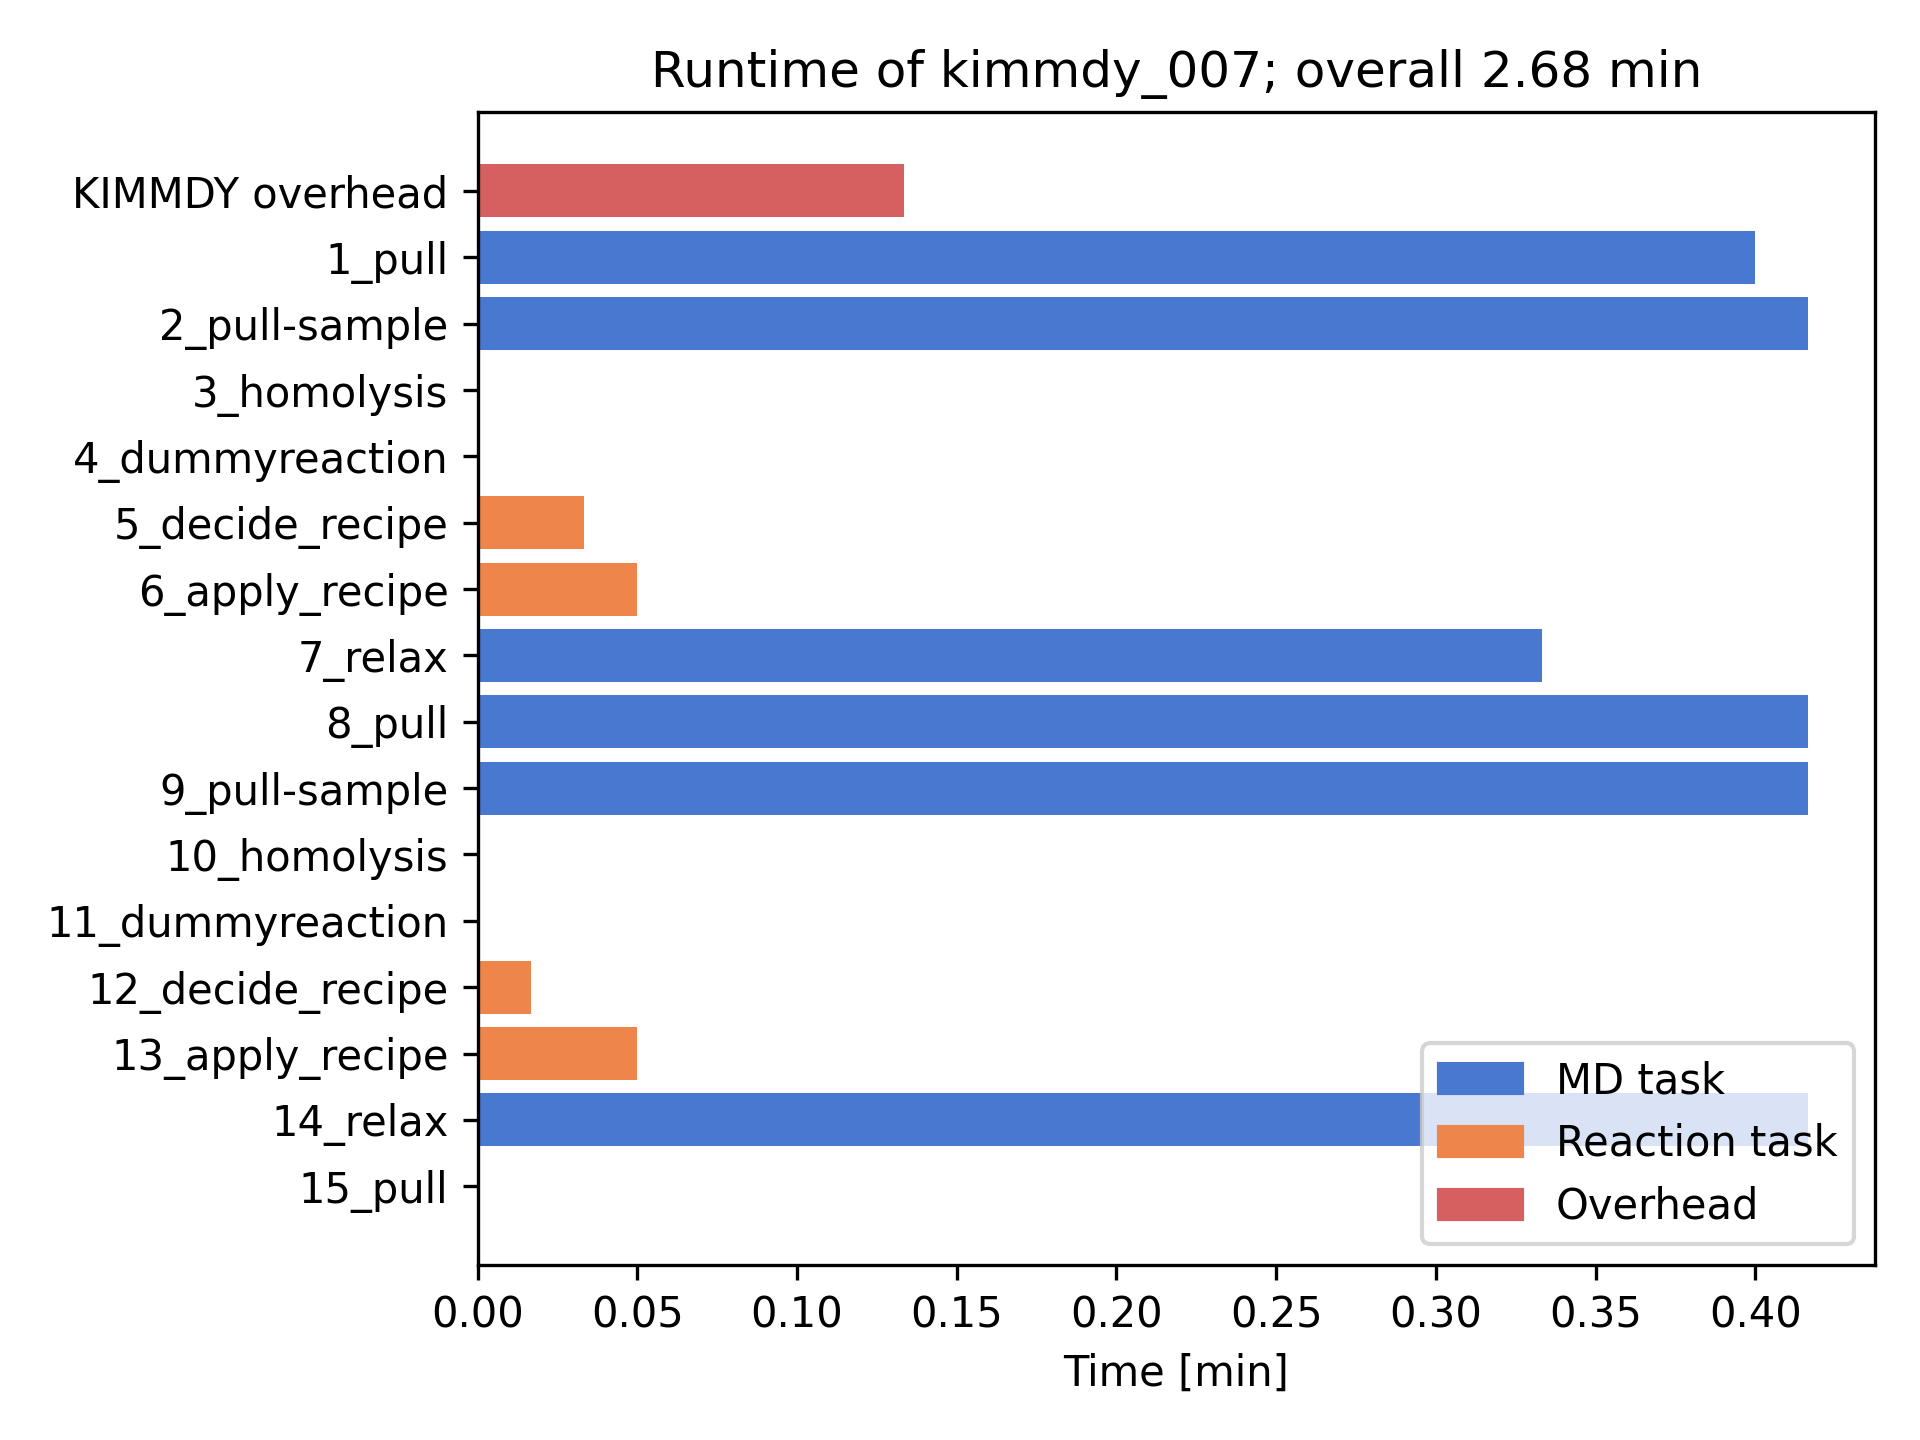
\includegraphics{www/tripelhelix_runtime.png}

\hypertarget{kimmdy-can-simulate-hats}{%
\subsection{KIMMDY can simulate HATs}\label{kimmdy-can-simulate-hats}}

\hypertarget{intramolecular-energy-behaves-almost-physically-correct}{%
\subsection{Intramolecular energy behaves almost physically
correct}\label{intramolecular-energy-behaves-almost-physically-correct}}

\texttt{kimmdy-analysis\ energy\ \textless{}run\_dir\textgreater{}\ -t\ Bond\ Angle\ Proper-Dih.}

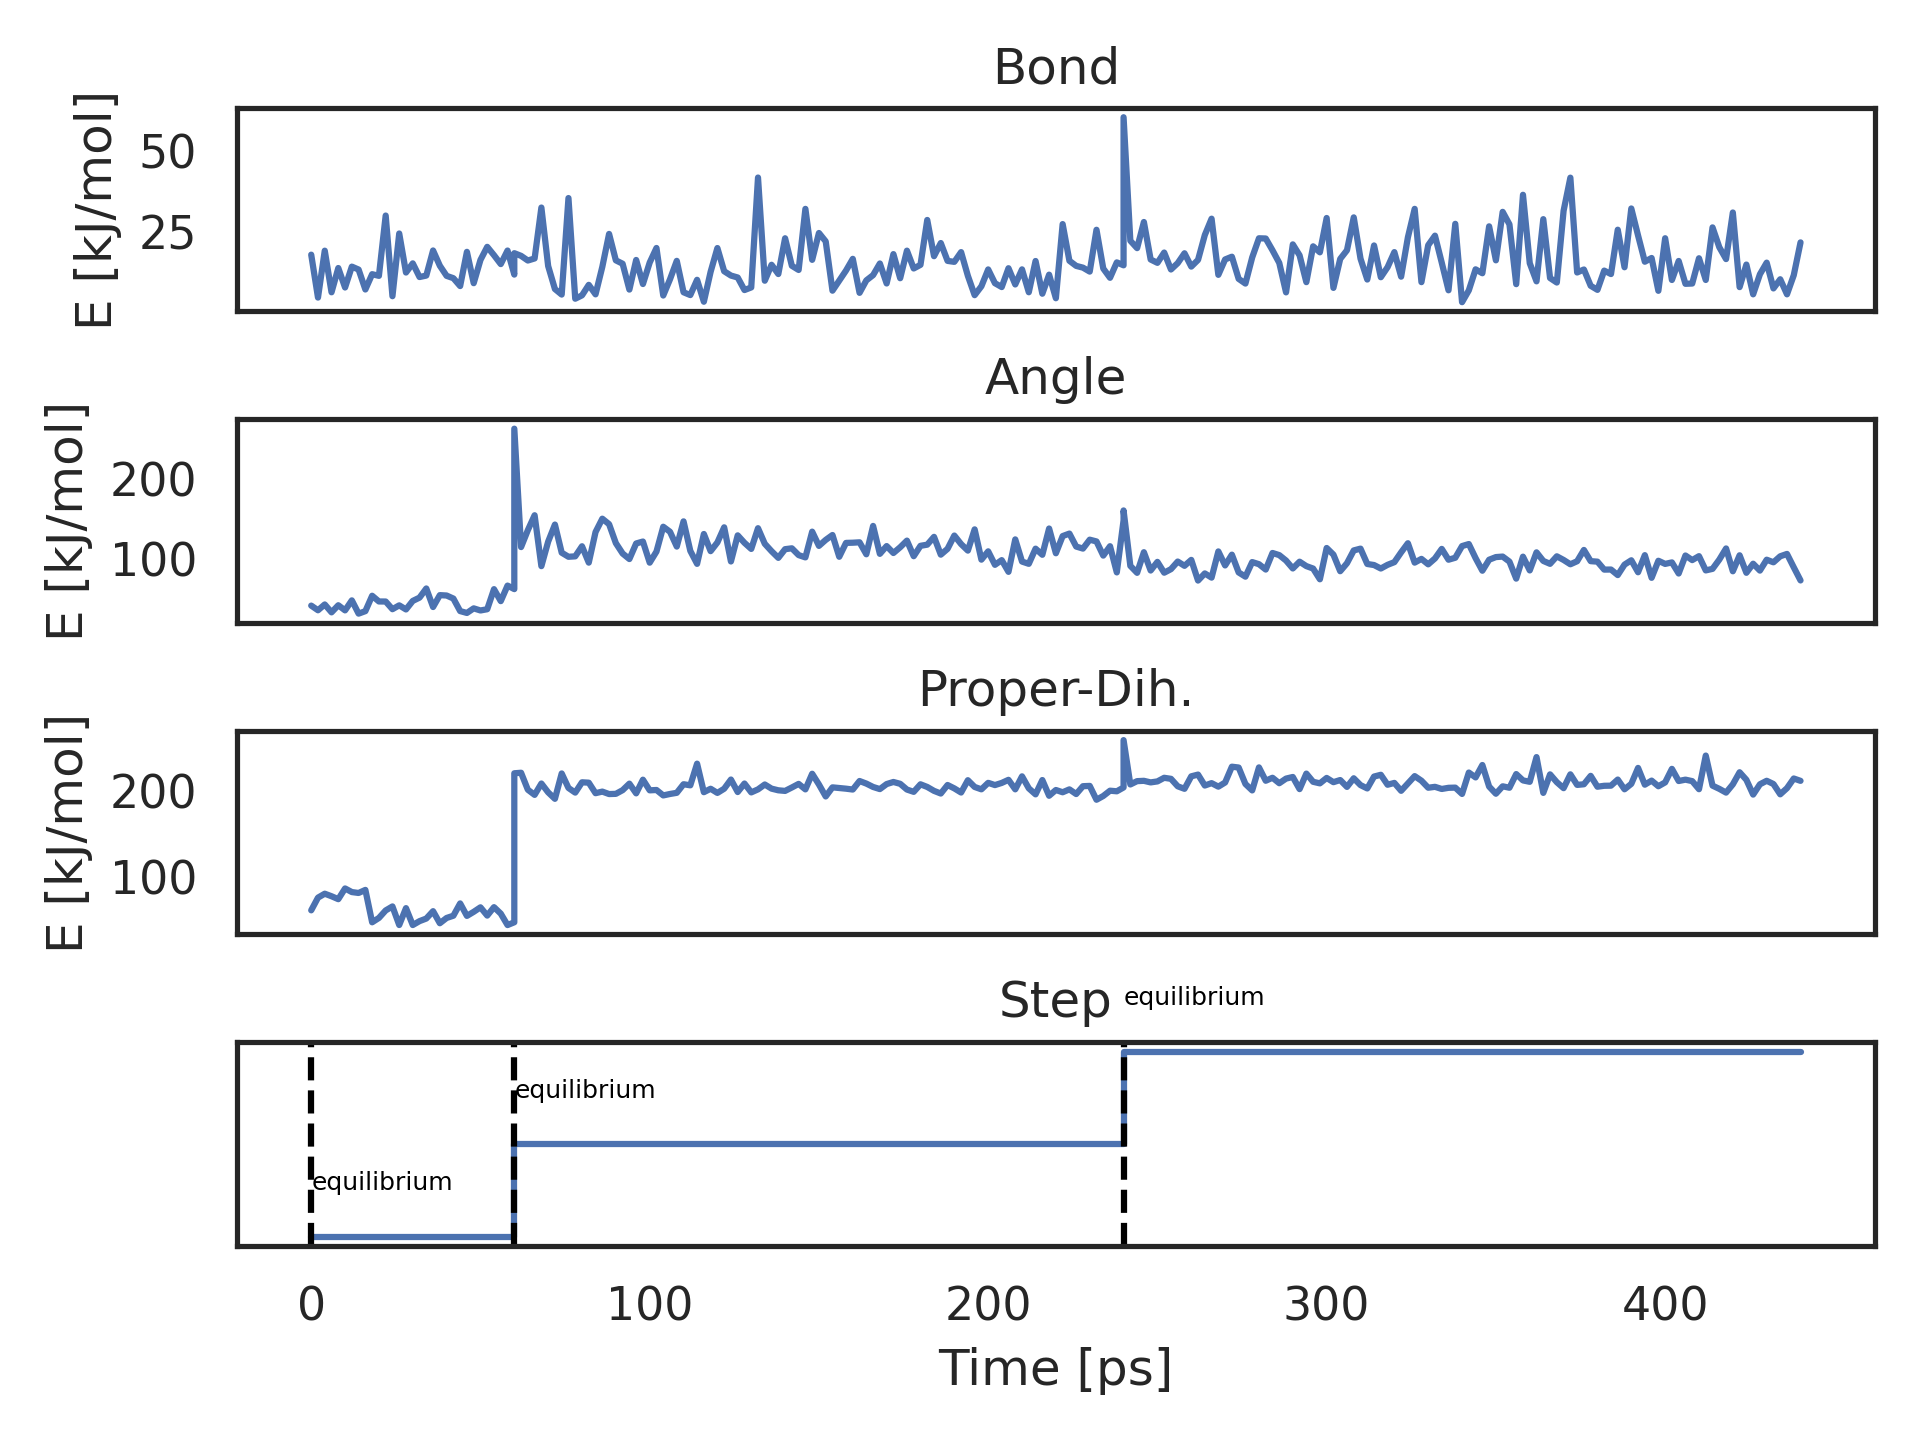
\includegraphics{www/ala_bonded.png}

\hypertarget{ml-models-increase-reaction-task-time}{%
\subsection{ML models increase reaction task
time}\label{ml-models-increase-reaction-task-time}}

\texttt{kimmdy-analysis\ runtime\ \textless{}run\_dir\textgreater{}}

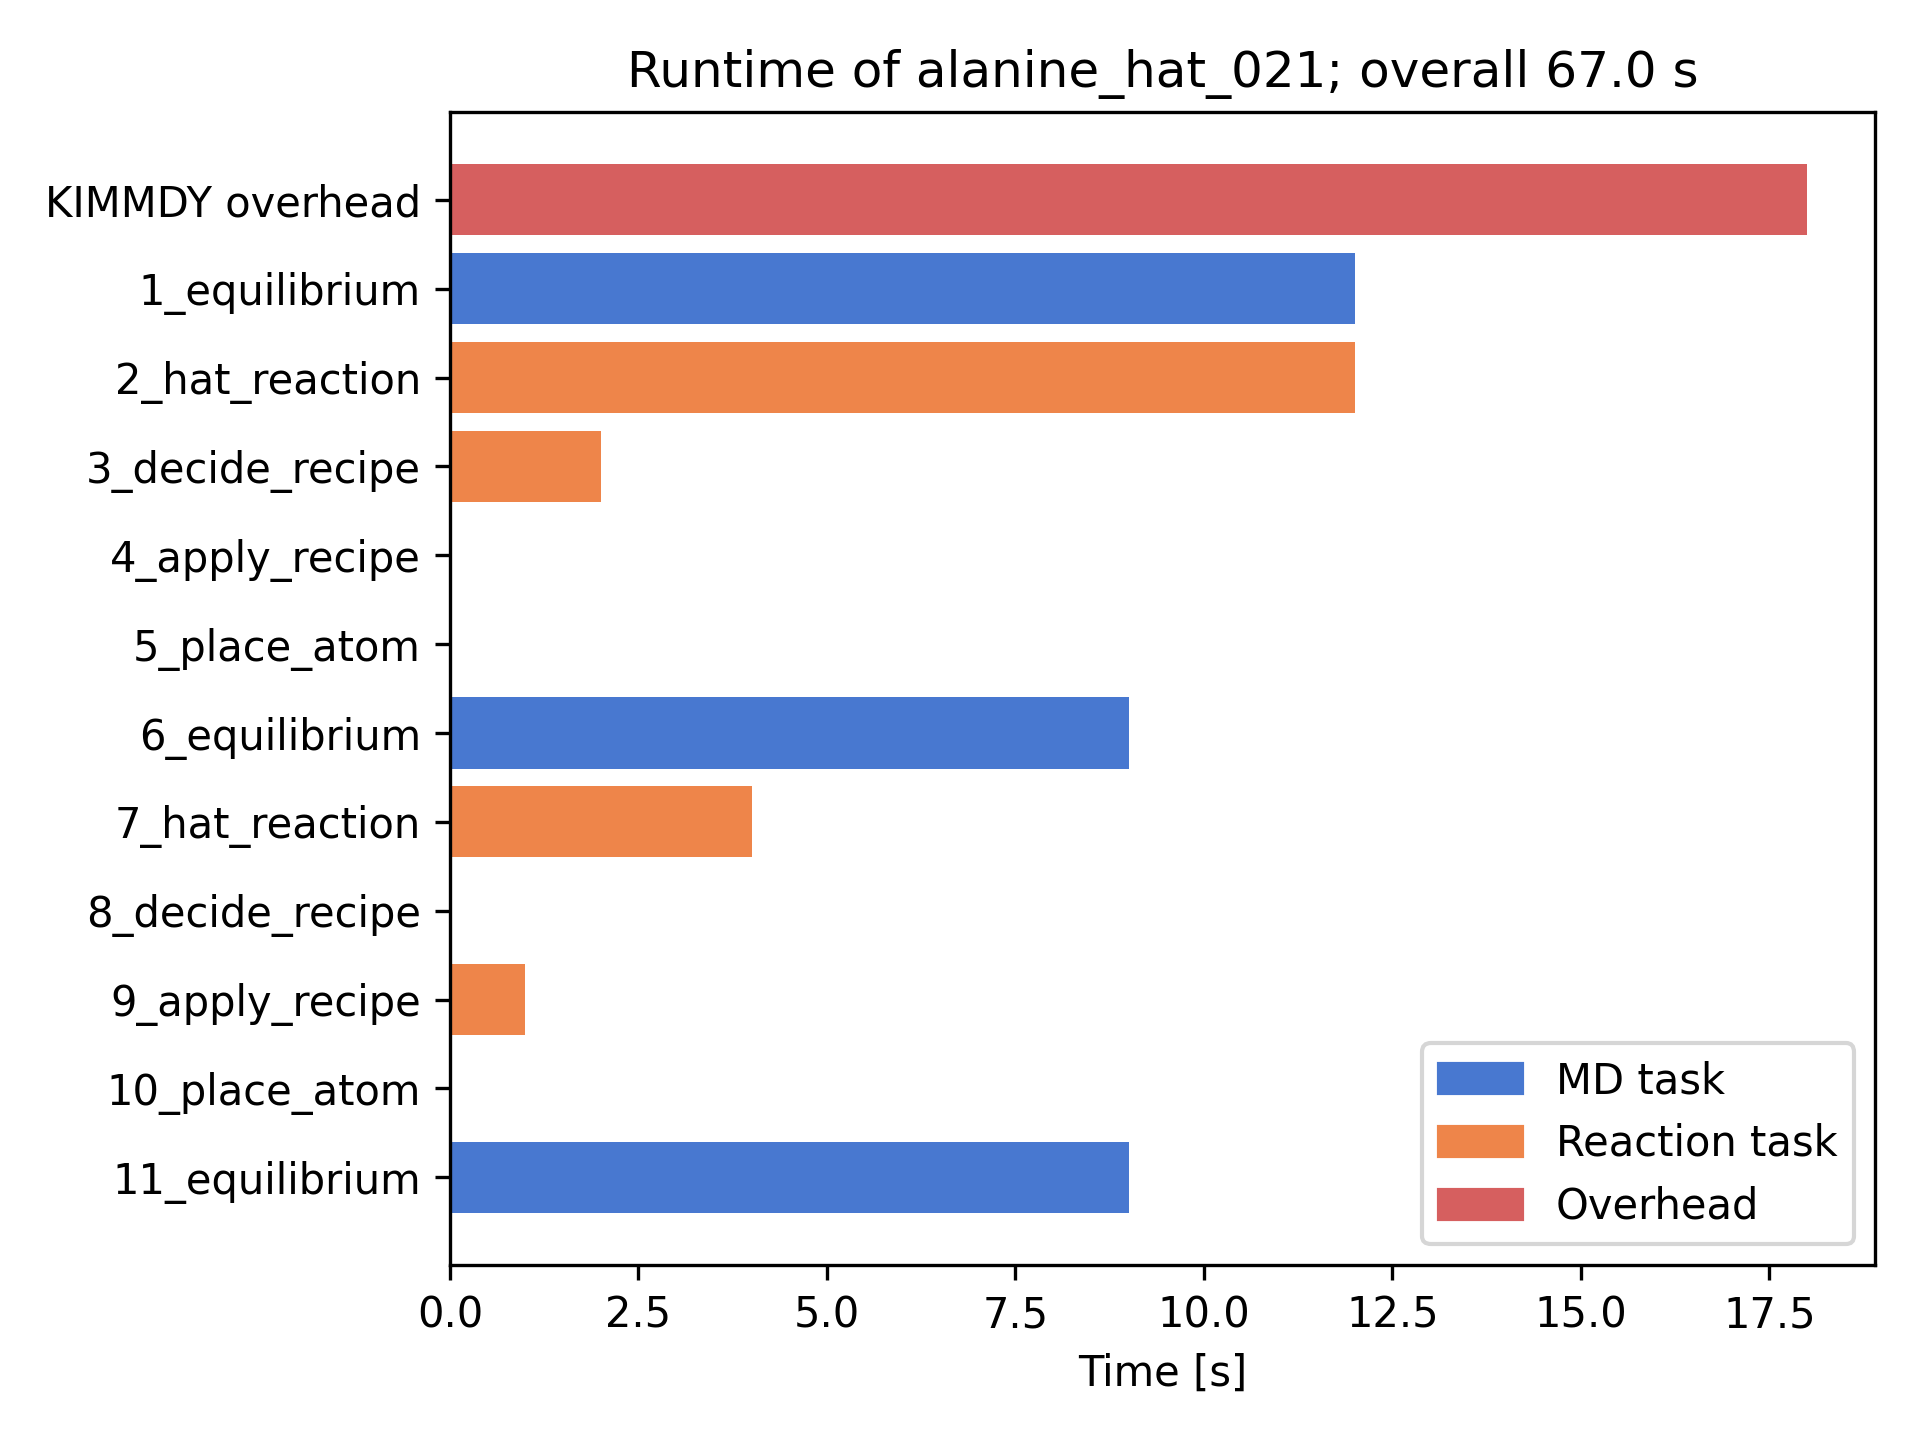
\includegraphics{www/ala_runtime.png}

\hypertarget{system-generation-is-semi-automated}{%
\subsection{System generation is
semi-automated}\label{system-generation-is-semi-automated}}

\texttt{pepgen\ A\ ala/}

\hypertarget{system-generation-is-semi-automated-1}{%
\subsection{System generation is
semi-automated}\label{system-generation-is-semi-automated-1}}

\texttt{kimmdy-remove-hydrogen\ pep.gro\ topol.top\ 14\ -p\ -e}

\hypertarget{conclusion}{%
\subsection{Conclusion}\label{conclusion}}

\begin{itemize}
\tightlist
\item
  KIMMDY v2 is mostly done
\item
  All aspects of the reaction functionality have been revisited
\item
  Theoretical foundations of KIMMDY are clear
\item
  Practicality of these simulations remains to be shown
\end{itemize}

\hypertarget{thank-you}{%
\section{Thank You!}\label{thank-you}}



\end{document}
